\documentclass[12pt, a4paper]{article}
\usepackage[utf8]{inputenc}
\usepackage{graphicx}
\usepackage{gensymb}
\usepackage{amsmath}
\usepackage{float}
\usepackage{subcaption}
\usepackage{caption}


\title{Eigen boundary value problems with}
\author{Miha Pompe}
\date{December 2021}

\begin{document}
\begin{titlepage}
	\centering
 	
\includegraphics[width=0.45\textwidth]{logo_fmf_uni-lj_sl_veliki.png}\par\vspace{1cm}

	\vspace{1cm}

	\vspace{1.5cm}
	{\huge\bfseries Eigen boundary value problems with\par}
	\vspace{2cm}
	{\Large Miha Pompe 28191072\par}
	\vfill

	\vfill

% Bottom of the page
	{\large December 2021\par}
\end{titlepage}
% \maketitle
\thispagestyle{empty}
\clearpage
\pagenumbering{arabic}
\newpage


\section{Introduction}

Given a differential equation and a few boundary values we can solve a boundary value problem. If this is an eigen problem we will have to compute the eigen values and vectors at the same time. Numerically we will be solving stationary Schrodinger's equation

\begin{equation*}
    -\frac{\hbar}{2m^2}\frac{d^2\psi}{dt^2} + V(x)\psi = E\psi
\end{equation*}

for infinite ($V(|x| < a/2) = 0$ and $V(|x| > a/2) = \infty$) and finite ($V(|x| < a/2) = 0$ and $V(|x| > a/2) = V_0$) potential well. For simplicity we can set $\hbar/2m = 1$.

\section{Infinite potential well}
The solutions for the infinite potential well are trigonometric functions.
\begin{equation*}
    \psi_n(x) = \sqrt{\frac{2}{a}} sin(k_n x) \quad k_n = \frac{n\pi}{a}
\end{equation*}
The energy of a state is given as $E_n = \frac{n^2\pi^2\hbar^2}{2mL^2}$ or in our simplified version $E_n = \frac{n^2\pi^2}{L^2}$. Here $n = 1,2,3,4,...$.

Numerical solutions will be calculated with two different methods, shooting method and finite differences method. The shooting method converts the BVP to an IVP where we are trying to find the optimal $\psi'(a)$ for the given boundary conditions. We first solve the IVP with an estimate of the derivative and then we iteratively change it to find the solution that satisfies the right side condition. 

\begin{figure}[hbtp]
  \begin{center}
  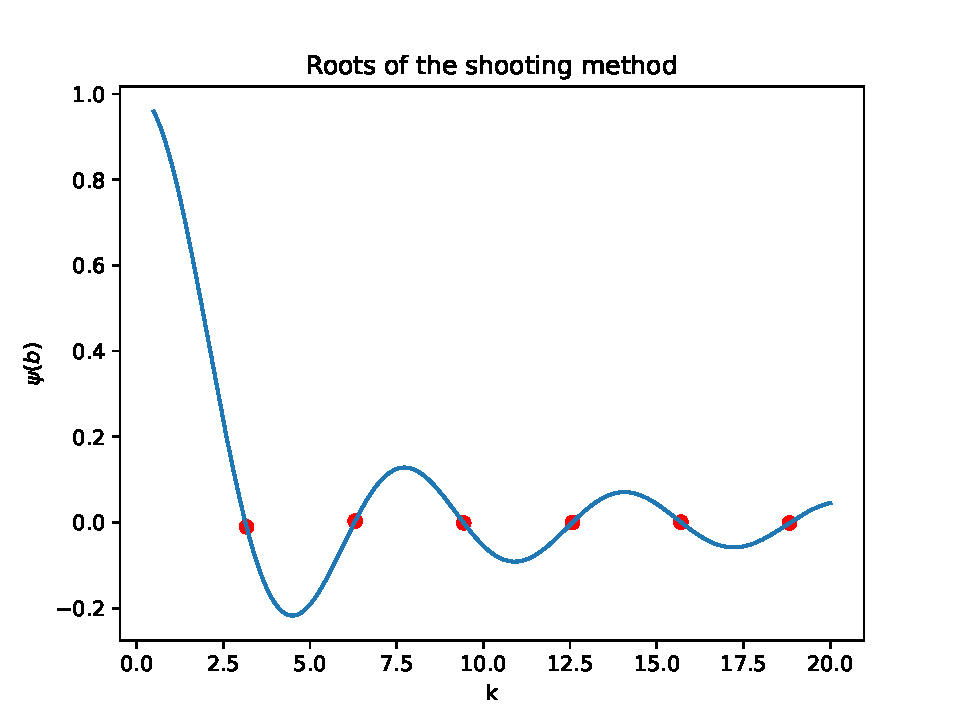
\includegraphics[width=7cm]{roots.pdf}
  \end{center}
  \vspace*{-7mm}
  \caption{Roots of $\psi(b, k)$, where $E = k^2$}
\end{figure}

The problem that arises with our problem is that the entire process is dependent on the eigen value ($E$). Therefore we first calculate the eigen values by finding roots for the function $\psi(b, E)$, as can be seen on Figure 1.

\begin{figure}[hbtp]
  \begin{subfigure}{0.5\textwidth}
  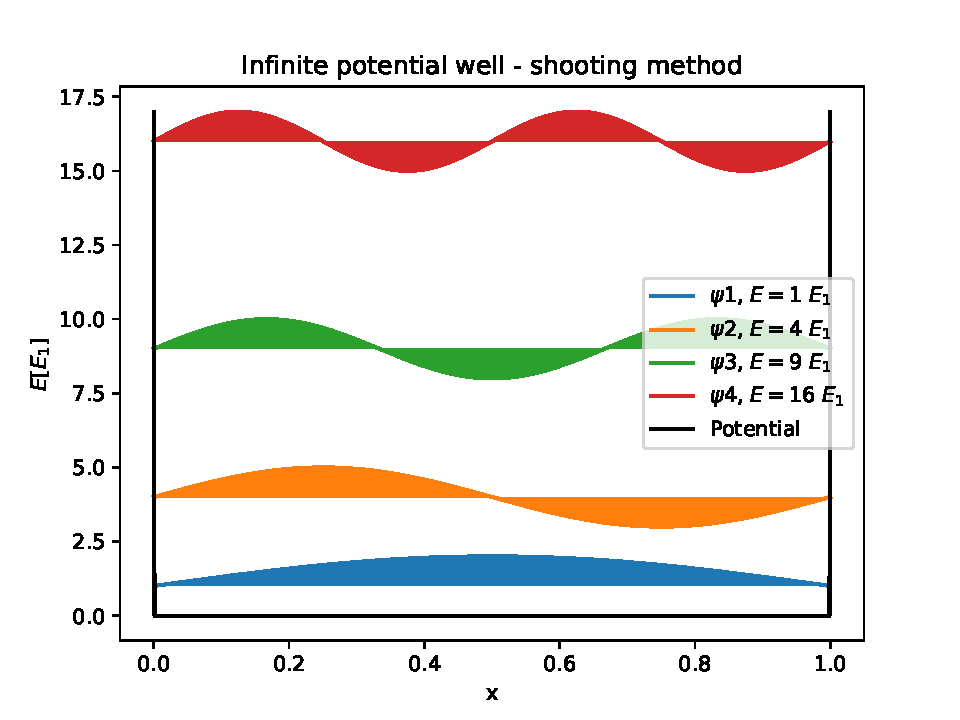
\includegraphics[width=\linewidth]{shoot_infinite.pdf}
  \caption{Infinite potential well solutions} \label{fig:a}
  \end{subfigure}
  \hspace*{\fill}
  \begin{subfigure}{0.5\textwidth}
  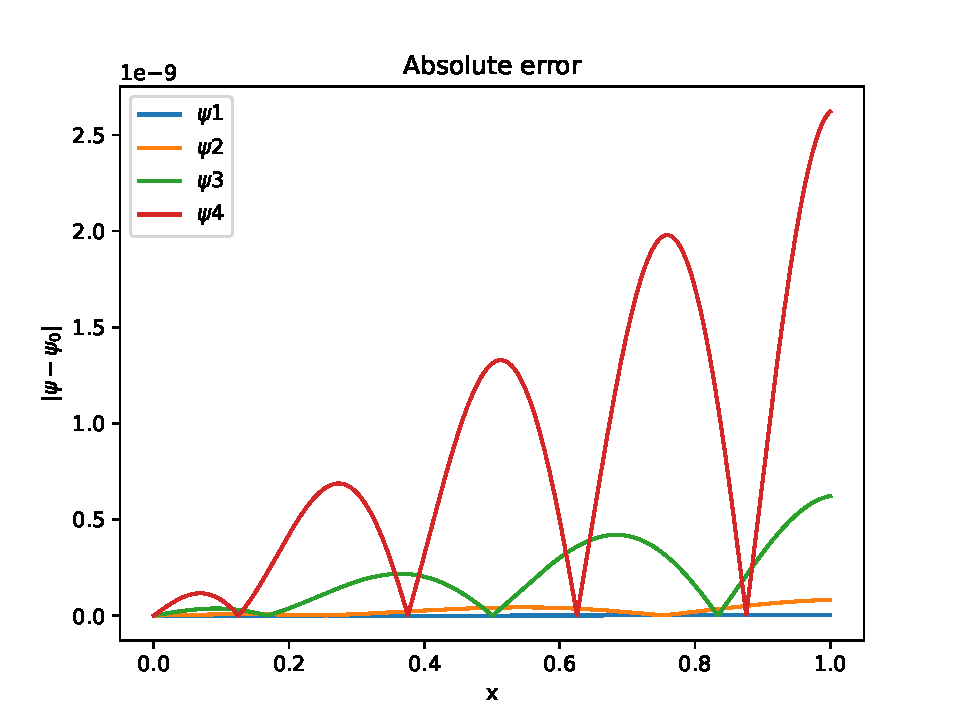
\includegraphics[width=\linewidth]{error_shoot_infinite.pdf}
  \caption{Absolute error of the numerical solution} \label{fig:b}
  \end{subfigure}
  \medskip
  \begin{subfigure}{0.5\textwidth}
  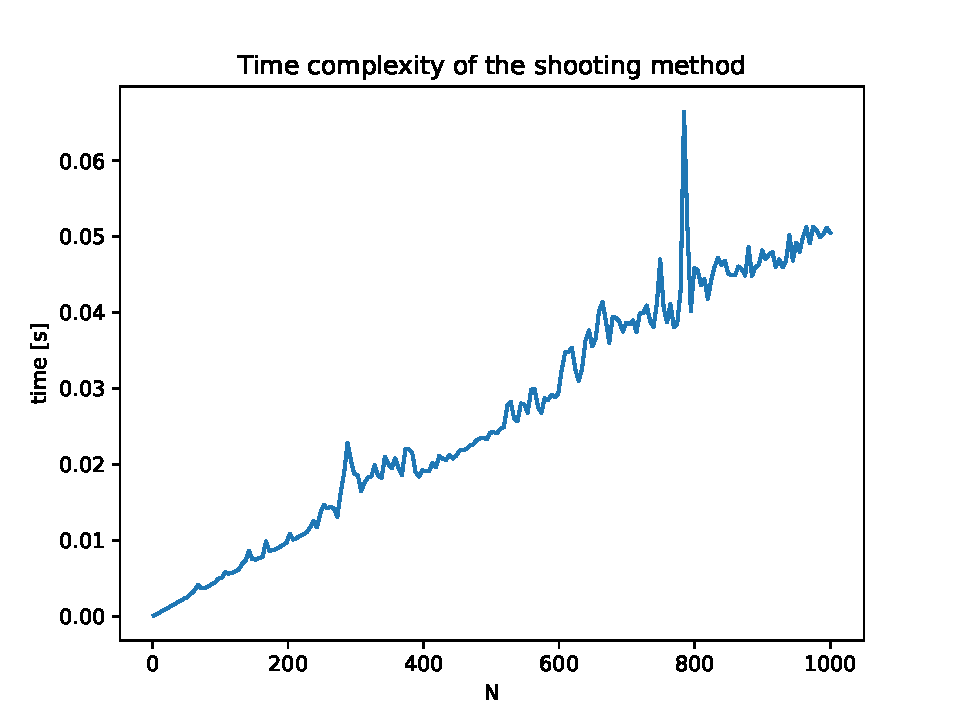
\includegraphics[width=\linewidth]{time_complexity_shoot.pdf}
  \caption{Time complexity in relation to number of steps} \label{fig:c}
  \end{subfigure}
  \hspace*{\fill}
  \begin{subfigure}{0.5\textwidth}
  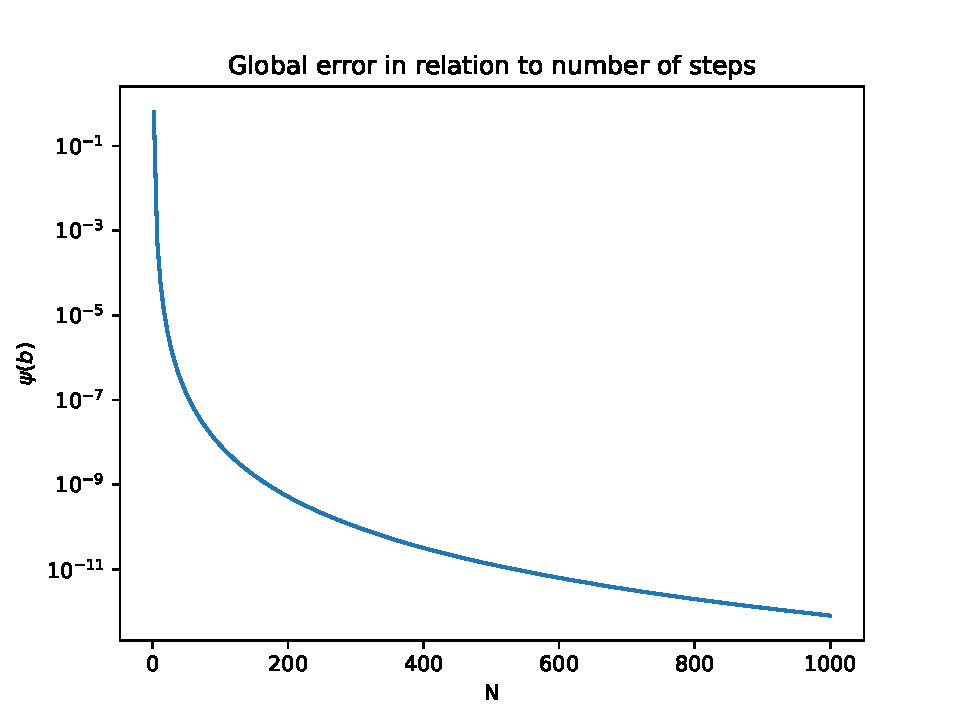
\includegraphics[width=\linewidth]{error_N.pdf}
  \caption{Global error in relation to number of steps} \label{fig:d}
  \end{subfigure}
%   \medskip
%   \begin{subfigure}{\textwidth}
%   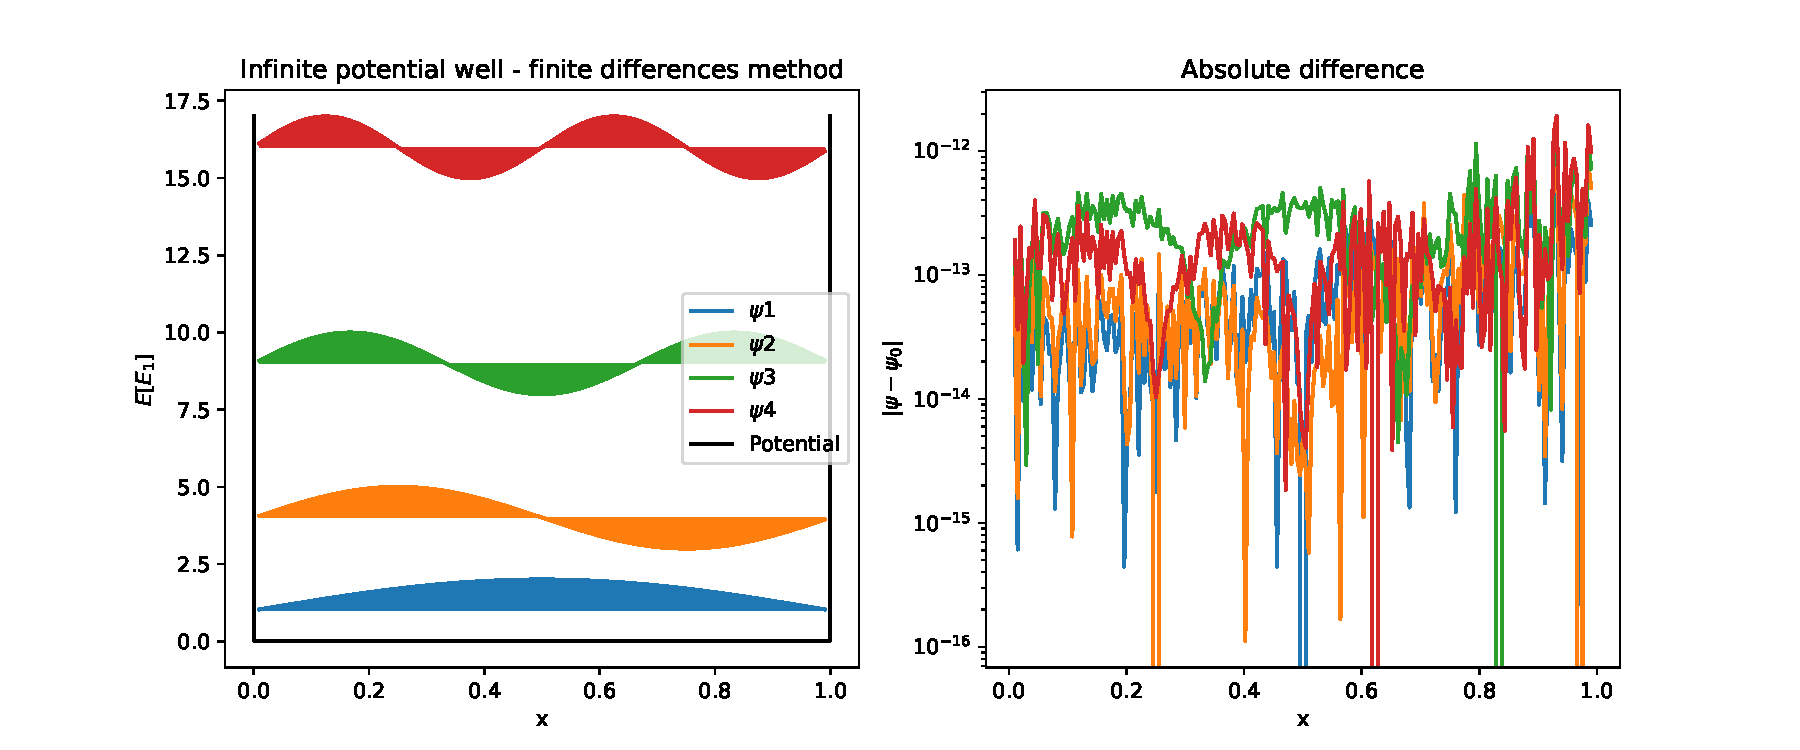
\includegraphics[width=\linewidth]{differences_infinite.pdf}
%   \caption{Lastne energije različnih potencialov. Desni graf je približana verzija levega.} \label{fig:e}
%   \end{subfigure}\hspace*{\fill}  
  \caption{Analysis of the shooting method for infinite potential well} \label{fig:1}
\end{figure}
 
The found energies increase quadratically, which is what we expect from theory. Using those energies we use the shooting method to calculate the eigen functions (Figure 2a). To compute the IVP we used fourth order Runge-Kutta. In Figure 2b we compare the numerical solution to the analytical one. The error increases with energy, which is the result of higher curvature at higher energies at constant step size. Secondly the error increases with position, which comes from the nature of the shooting method, which propagates the solution from left to right. The highest error occur at the roots of the solutions.

The second parameter we can alter is the number of points in the interval $[a, b]$, denoted with $N$. Figure 2c shows that the computation time increases linearly with $N$. Secondly we see from Figure 2d that the global error decreases exponentially with $N$.

\begin{figure}[hbtp]
  \begin{subfigure}{\textwidth}
  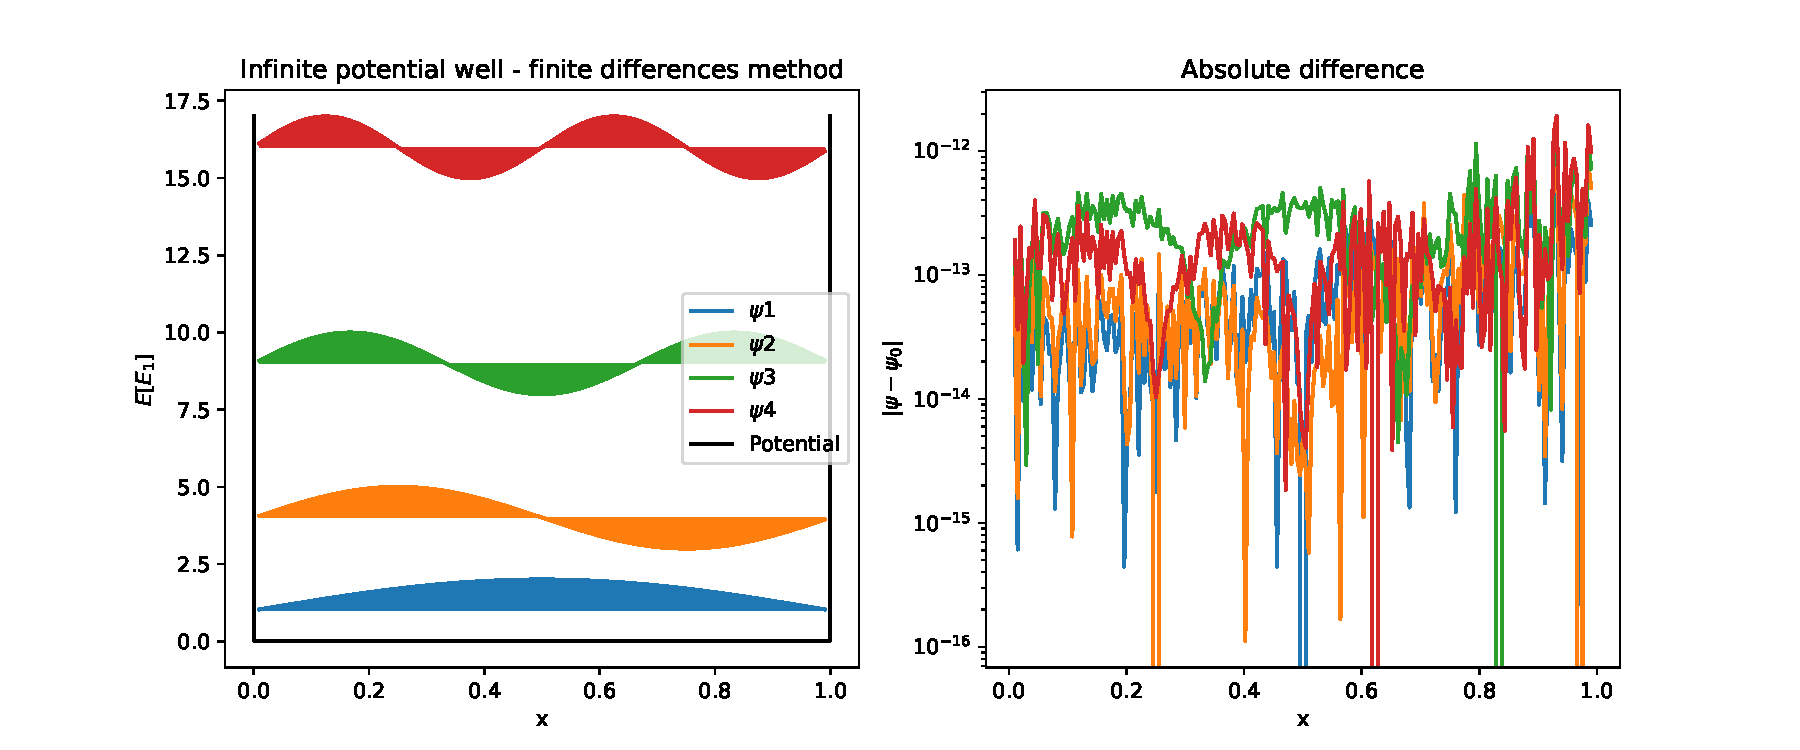
\includegraphics[width=\linewidth]{differences_infinite.pdf}
  \caption{Solutions using finite differences method and the absolute error compared to the analytical solution.} \label{fig:e}
  \end{subfigure}
  %\hspace*{\fill}
  \medskip
  %\hspace*{\fill}
  \begin{subfigure}{0.5\textwidth}
  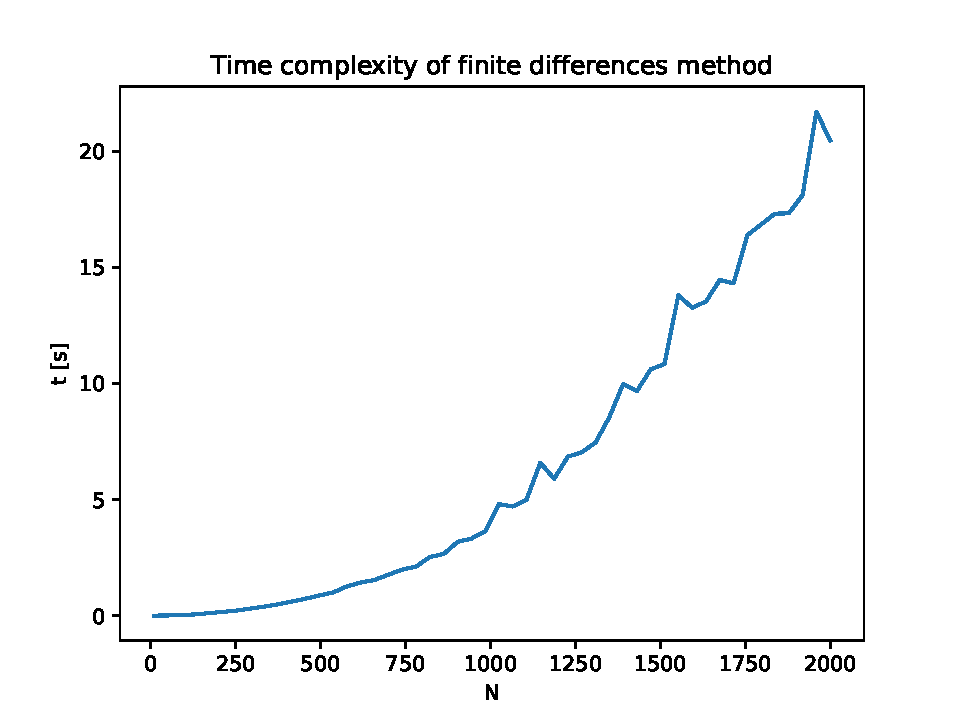
\includegraphics[width=\linewidth]{time_diff.pdf}
  \caption{Computation time in comparison to number of steps $N$} \label{fig:a}
  \end{subfigure}
  %\hspace*{\fill}
  \begin{subfigure}{0.5\textwidth}
  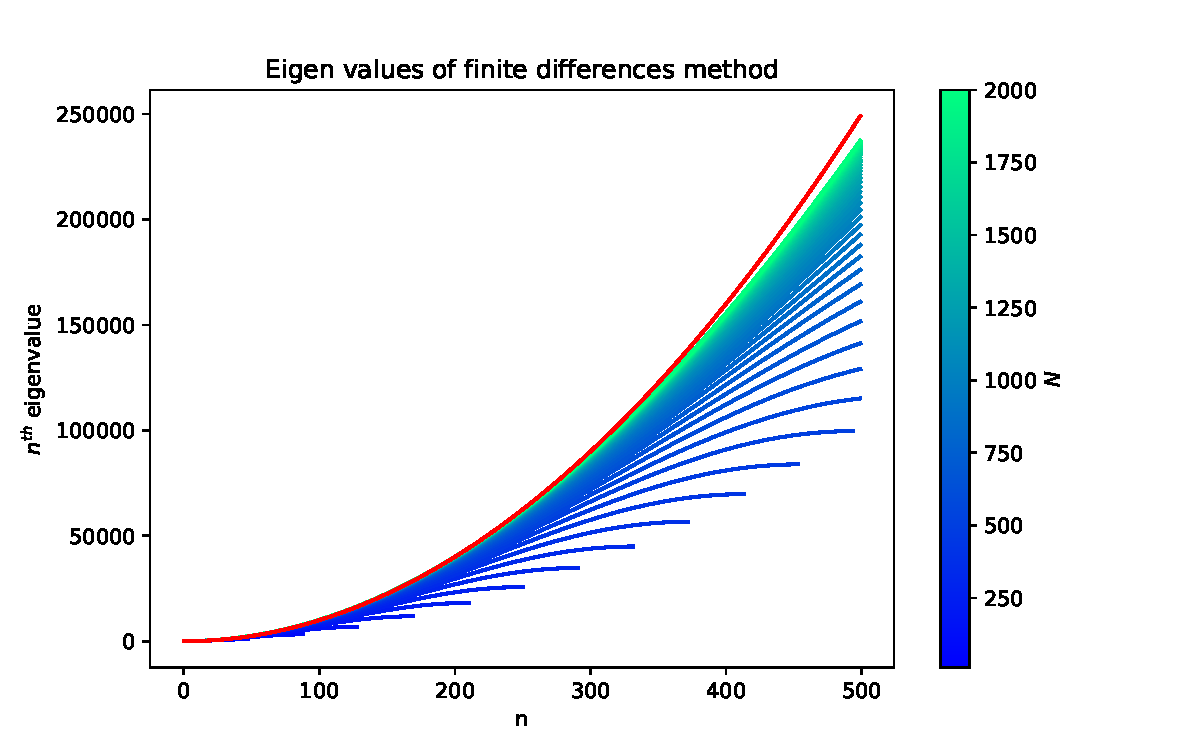
\includegraphics[width=\linewidth]{eigen_diff.pdf}
  \caption{Eigen values in comparison to number of steps $N$} \label{fig:b}
  \end{subfigure}
%   \medskip
%   \begin{subfigure}{0.5\textwidth}
%   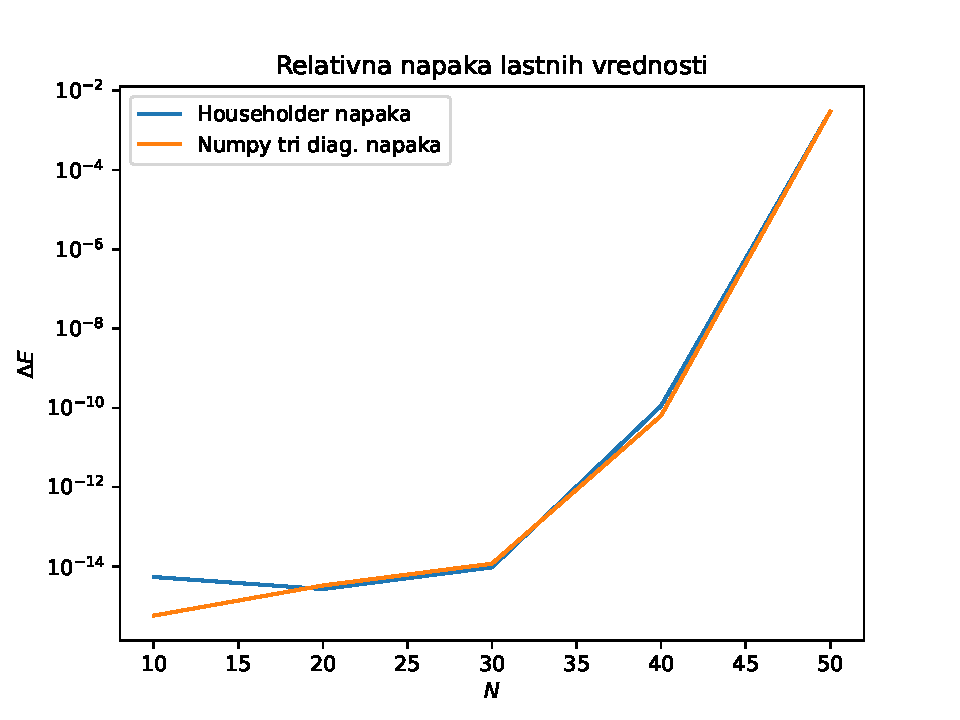
\includegraphics[width=\linewidth]{grafi/eigen_vs_N2.pdf}
%   \caption{Relativna napaka lastnih vrednosti manjših matrik.} \label{fig:c}
%   \end{subfigure}
%   \hspace*{\fill}
%   \begin{subfigure}{0.5\textwidth}
%   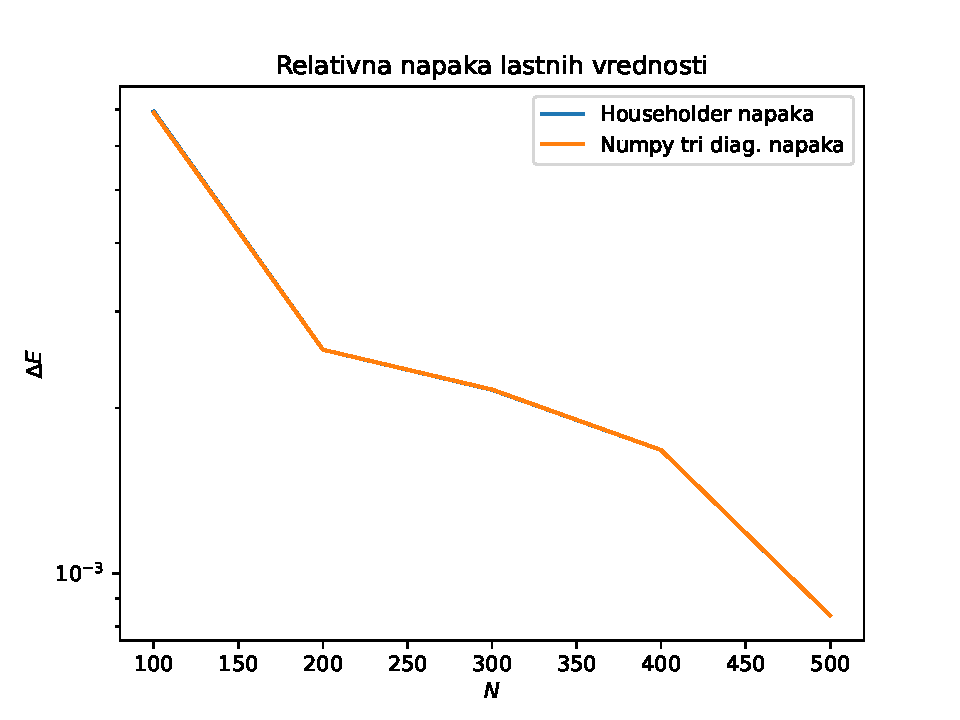
\includegraphics[width=\linewidth]{grafi/eigen_vs_N2_2.pdf}
%   \caption{Relativna napaka lastnih vrednosti večjih matrik.} \label{fig:d}
%   \end{subfigure}
  
\caption{Analysis of infinite potential well using finite differences method} \label{fig:1}
\end{figure}

Finite differences is the second method we will use to solve the problem. Here we rewrite the derivatives as finite difference of neighboring points. Schrodinger's equation can be rewritten in the following form

\begin{equation*}
    -\frac{\psi_{i-1}-2\psi_i + \psi_{i+1} }{h^2} + V(x_i)\psi_i = E\psi_i
\end{equation*}
which we can rewrite in therms of a system of linear equations $A\psi = E\psi$ where $A$ is:
\begin{equation*}
    A = -h^{-2}
    \begin{bmatrix}
    -2-h^2V(x_1)&1\\
    1&-2-h^2V(x_2)&1\\
    &&...\\
    &&1&-2-h^2V(x_{N-1})
    \end{bmatrix}
\end{equation*}

$A$ is a three diagonal matrix whose eigen values and vectors were computed using {\sc numpy.linalg.eig}. In this case the matrix can be further simplified as $V = 0$.

Figure 3a presents the solutions computed using the finite differences method and the error. The error does not stem from the method itself but from numerics. The error is also proportional to the number of points $N$.

Figure 3c analyses the accuracy of eigen values. We notice that smaller values closely match the theoretical values. Therefore if we want to accurately compute eigen values we must choose adequately high $N$.

The diagonalization algorithm used is not specialized for three diagonal matrices, therefore the time complexity is not linear, but polynomial, as can be concluded from Figure 3b.

\section{Finite potential well} 
 
Having derived formals for arbitrary potentials ($V(x)$) we can examine any example. In this part we focus on the finite potential well. The analytical solution is a combination of exponential and trigonometric functions. The solution is:

\begin{equation*}
    \psi = \begin{cases}
    Ae^{\kappa x}  & x < -a/2 \\
    Be^{ikx} + Ce^{-ikx} & |x| < a/2\\
    Ae^{-\kappa x} & x > a/2
    \end{cases}
\end{equation*}
where $k$ and $\kappa$ are solutions of the following equations:
\begin{equation*}
    tan\frac{u}{2} = \sqrt{\frac{u_0^2}{u^2}-1}\quad
    -cot\frac{u}{2} = \sqrt{\frac{u_0^2}{u^2}-1}
\end{equation*}
where $u = ka$ and $u_0 = \frac{2mV_0}{\hbar^2}$. The left equation gives us values for even functions and the right one for the odd functions. Afterwards we can calculate the constants $A$, $B$ and $C$.

Numerically we solve this problem as we did the infinite potential well, therefore let us just examine the solutions. If we expect Figure 4 we can observe exponential tails in both solutions and also appropriate oscillations in the middle.
 
\begin{figure}[hbtp]
  \begin{center}
  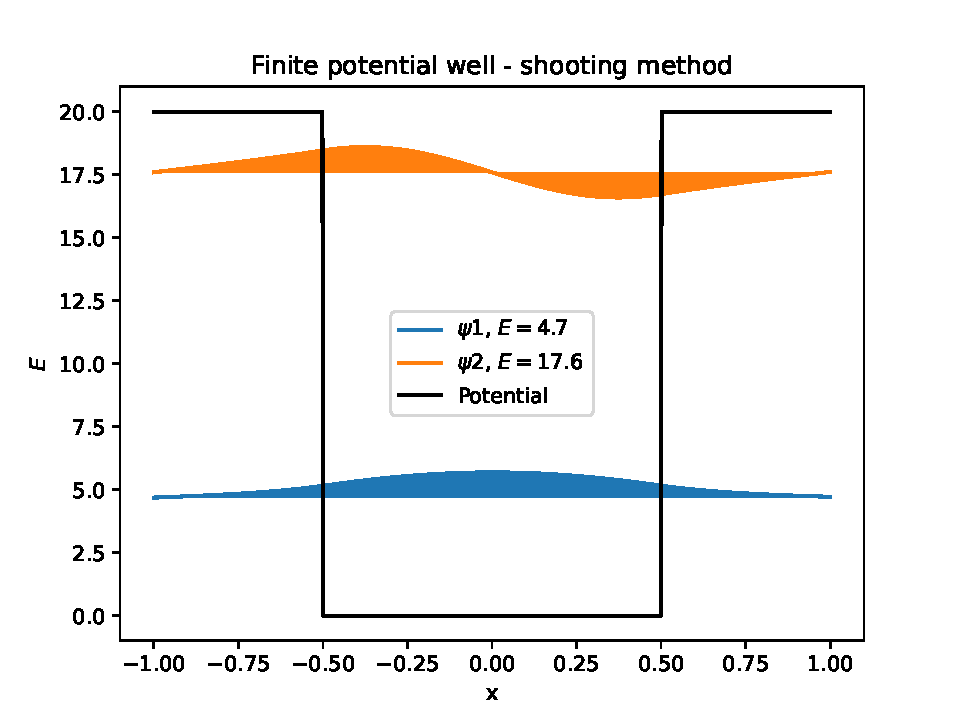
\includegraphics[width=10cm]{shoot_finite.pdf}
  \end{center}
  \vspace*{-7mm}
  \caption{Analysis of excited damped oscillator}
\end{figure}

\end{document}